% vim: set textwidth=78 autoindent:

\subsection{Complemento de exportaci�n a MapServer}\label{sec:mapserver_export}

% when the revision of a section has been finalized, 
% comment out the following line:
%\updatedisclaimer

Puede usar QGIS para ``dise�ar'' su mapa agregando y acomodando capas, 
simboliz�ndolas, personalizando los colores y entonces creando un archivo map
para MapServer.

\subsubsection{Creando un Archivo de Proyecto}

El complemento de Exportaci�n a MapServer opera en un proyecto de QGIS guardado  
\textbf{no} en el contenido actual del canvas del mapa y leyenda. Esto  
ha sido fuente de confusi�n para un n�mero de usuarios. Como se describe abajo, 
antes de iniciar usando el complemento de Exportaci�n a MapServer, necesita acomodar 
las capas raster y vectoriales que quiere usar en mapserver y guardar este estado
en un archivo de proyecto de QGIS.

\begin{figure}[ht]
\begin{center}
  \caption{Acomodar capas raster y vectoriales para un archivo de proyecto QGIS \nixcaption}
  \label{fig:mapserver_export_qgs}\smallskip
  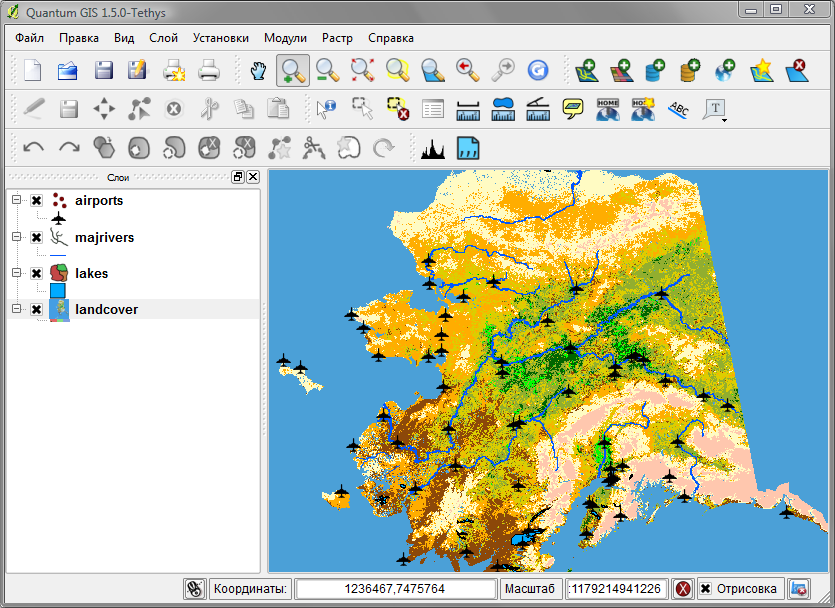
\includegraphics[clip=true, width=12cm]{mapserver_export_qgis}
\end{center}
\end{figure}

En este ejemplo, demostramos los cuatro pasos requeridos para crear un proyecto
simple el cual puede ser usado para crear el archivo map de Mapser. 
Usamos archivos raster y vectoriales desde el conjunto de datos de ejemplo de QGIS \ref{label_sampledata}.

\begin{enumerate}
\item Agregue la capa raster \filename{landcover.tif} haciendo clic en el �cono 
\toolbtntwo{mActionAddRasterLayer}{A�adir capa Raster}.
\item A�ada los Shapefiles \filename{lakes.shp, majrivers.shp} y 
\filename{airports.shp} del conjunto de datos de QGIS haciendo clic en el �cono 
\toolbtntwo{mActionAddNonDbLayer}{A�adir capa vectorial}.
\item Cambie los colores y simbolice los datos como lo desee (por ejemplo vea la 
figura~\ref{fig:mapserver_export_qgis})
\item Guarde un nuevo proyecto llamado \filename{mapserverproject.qgs} usando 
\mainmenuopt{Archivo} > \dropmenuopttwo{mActionFileSave}{Guardar proyecto}.
\end{enumerate} 

\subsubsection{Creando el archiv Map}

La herramiente para exportar \filename{msexport} un proyecto de QGIS a un map de MapServer 
est� instalada en su directorio de binarios de QGIS y puede ser usado de forma independiente de QGIS. 
Para usarla dentro de QGIS, necesita activar el complemento de Exportaci�n a MapServer usando el administrador de complementos (vea la secci�n \ref{sec:load_core_plugin}).

\begin{figure}[ht]
\begin{center}
  \caption{Di�logo Exportar a MapServer  \nixcaption}
  \label{fig:mapserver_export_dialog}\smallskip
  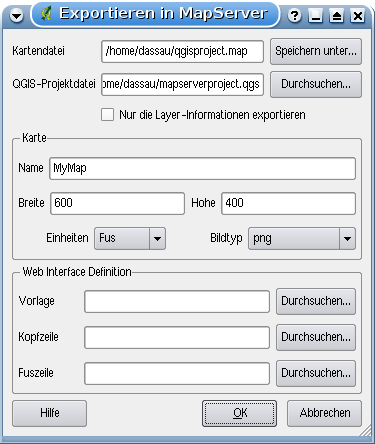
\includegraphics[clip=true, width=9cm]{mapserver_export_dialog}
\end{center}
\end{figure}

\begin{description}
\item [Archivo de Mapa] \mbox{}\\
Escriba el nombre del archivo de mapa a ser creado. Puede usar el bot�n a la derecha para explorar
para localizar el directorio donde desea que el archivo de mapa sea creado. 
\item [Archivo de proyecto de Qgis] \mbox{}\\
Escriba la ruta completa al archivo de proyecto de QGIS (.qgs) que desea exportar. Puede usar el bot�n 
a la derecha para localizar el archivo de proyecto de QGIS.
\item [Nombre del Mapa] \mbox{}\\
Un nombre para el mapa. Este nombre es usado como prefijo para todas las im�genes generadas por mapserver.
\item [Anchura del Mapa] \mbox{}\\
Ancho de la imagen de salida en pixeles.
\item [altura del Mapa] \mbox{}\\
Altura de la imagen de salida en pixeles.
\item [Unidades del Mapa] \mbox{}\\
Unidades de medida usadas para la salida.
\item [Tipo de Imagen] \mbox{}\\
Formato para la imagen de salida generada por MapServer.
\item [Plantilla Web] \mbox{}\\
Ruta completa al archivo de plantilla de MapServer a ser usada con el archivo de mapa.
\item [Encabezado Web] \mbox{}\\
Ruta completa al archivo de encabezado de MapServer a ser usado con el archivo de mapa.
\item [Pie de P�gina Web] \mbox{}\\
Ruta completa al archivo de pie de p�gina de MapServer a ser usado con el archivo de mapa.
\end{description}

Solo las entradas de \filename{archivo de Mapa} y \filename{archivo de proyecto de QGIS} son 
requeridos para crear el archivo de mapa, sin embargo omitiendo los otros par�metros, 
puede terminar en la creaci�n de un archivo de mapa no funcional, dependiendo del uso que se pretende. 
Aunque QGIS es bueno creando un archivo de mapas de su archivo de proyecto, 
puede requerir de algunos ajustes para obtener los resultados que desea. 
Para este ejemplo, crearemos un archivo de mapa usando el archivo de proyecto 
\filename{mapserverproject.qgs} que creamos
(vea la figura~\ref{fig:mapserver_export_dialog}):

\begin{enumerate}
  \item  Iniciar el di�logo de MapServer (vea la  
figura \ref{fig:mapserver_export_dialog}) haciendo clic en el �cono \toolbtntwo{mapserver_export}{Exportar a MapServer} del men� de herramientas.
  \item Escriba el nombre (ej., \filename{qgisproject.map}) para su nuevo archivo de mapa.
  \item Explore y encuentre el archivo de proyecto de QGIS (ej., \filename{mapserverproject.qgs}) 
  que previamente guardo.
  \item Escriba un nombre (ej., \filename{MiMapa}) para el mapa.
  \item Escriba la anchura y altura (ej., \filename{600} para el ancho y \filename{400} para la altura)para su imagen de salida.
  \item Para este ejemplo, las capas est�n en metros, de manera que cambiamos las unidades a metros.
  \item Elija ``png'' para el tipo de imagen.
  \item Clic \button{OK} para generar el nuevo archivo de mapa \filename{qgisproject.map}. 
  QGIS muestra el �xito de sus esfuerzos.
\end{enumerate}

Puede ver el archivo de mapa en cualquier editor de texto o visualizar. Si le echa un vistazo,
notar� que la herramienta para exportar le agrega los metadatos necesarios
para activar nuestro mapa como WMS. 

\subsubsection{Probando su archivo de mapa}

Ahora podemos probar nuestro trabajo usando la herramiente \filename{shp2img} para crear una imagen desde el archivo de mapa. La utiler�a \filename{shp2img} es parte de MapServer y FWTools. 
Para crear una imagen de nuestro mapas:

\begin{itemize}
\item Abrir una terminal
\item Si no ha almacenado su archivo de mapa en su directorio home, cambiese al
  directorio donde lo almaceno.
\item Ejecute \filename{shp2img -m qgisproject.map -o mapserver\_test.png} y 
  muestre la imagen. 
\end{itemize}
 
Esto crea un PNG con todas las capas incluidas en el archivo de proyecto de QGIS. 
Adem�s, la extensi�n del PNG ser� la misma que cuando guardamos el proyecto.
Como puede ver en la figura~\ref{fig:mapserver_export_test}, toda la  
informaci�n excepto los s�mbolos de aeropuertos son incluidos.

\begin{figure}[ht]
\begin{center}
  \caption{PNG de prueba creado con shp2img con todas las capas exportadas a MapServer \nixcaption}
  \label{fig:mapserver_export_test}\smallskip
  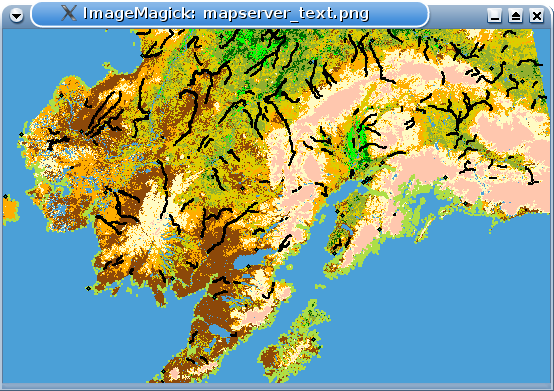
\includegraphics[clip=true, width=12cm]{mapserver_export_test}
\end{center}
\end{figure}

Si planea usar el archivo de mapa para servir requerimientos WMS, probablemente no
tiene que ajustar nada. Si planea usarlo con una plantilla de mapeo o una
interface, puede tener que realizar un poco de trabajo manual. Para ver que tan facil
es ir de QGIS a servir mapas en el web, vea el video de
5 minutos de Christopher Schmidt. El us� una versi�n vieja de QGIS (versi�n 0.8), pero el demo aplica
igualmente a las versiones mas recientes.
\footnote{\url{http://openlayers.org/presentations/mappingyourdata/}}
